\documentclass[12pt]{book}
\usepackage{cdt/cdtBusiness}
\usepackage{requerimientos}
\usepackage{paear}
\usepackage{subfigure}
\usepackage[spanish]{babel}
\usepackage{rotating}
\usepackage{tabulary}
\usepackage{makecell}
\usepackage{listings}
\usepackage{pdfpages}
%\usepackage[nosectionbib]{apacite}
%\usepackage[square,numbers]{natbib}
%%%%%%%%%%%%%%%%%%%%%%%%%%%%%%%%%%%%%%%%%%%%%%%%%%%%%%%%%%%%%%%%
% Datos del proyecto

\organizacion[]{Escuela Superior de Cómputo}
\autor[]{Instituto Politécnico Nacional}
\sistema[]{Sistema de Monitoreo de Signos Vitales Utilizando IoT}
\proyecto[]{}
\documento{}{Documento Técnico}%{\RELEASE{1.0}}%{\DRAFT{\today}} 

\entregable{}{\Large{Sistema de Monitoreo de Signos Vitales Utilizando IoT}} 

% Descomentar y establecer la fecha cuando se desee congelar la fecha del documento.
%\fecha{12 de Abril de 2013}

%%%%%%%%%%%%%%%%%%%%%%%%%%%%%%%%%%%%%%%%%%%%%%%%%%%%%%%%%%%%%%%%
% Datos para revisión
%\elaboro[Alumnos de la Licenciatura en Ingeniería en Sistemas Computacionales IPN - ESCOM]{Cesar Raúl Avila Padilla\vspace{0.4cm} Ivo Sebastián Sam Álvarez-Tostado\vspace{0.4cm}} % Responsable del contenido (IPN) Lic. Ulises Vélez Saldaña
%\superviso[Alumnos de la Licenciatura en Ingeniería en Sistemas Computacionales IPN - ESCOM]{Cesar Raúl Avila Padilla\vspace{0.4cm} Ivo Sebastián Sam Álvarez-Tostado\vspace{0.4cm}}
%\aprobo[Directores del Trabajo Terminal 2017-A108]{M. en C. Ulises Velez Saldaña\\ M. en C. José David Ortega Pacheco} % Responsable Técnico (Contraparte)

%\title{\varProyecto}
%\subtitle{\varCveDocumento--\varDocumento}


%%%%%%%%%%%%%%%%%%%%%%%%%%%%%%%%%%%%%%%%%%%%%%%%%%%%%%%%%%%%%%%%
% Documentos relacionados con el documento actual

% TODO: Escriba los documentos en los que está basado este documento.

%%%%%%%%%%%%%%%%%%%%%%%%%%%%%%%%%%%%%%%%%%%%%%%%%%%%%%%%%%%%%%%%
% Elementos contenidos en el documento

% TODO: Al finalizar el análisis resuma aquí todos los elementos del componente: RN, CU, IU, MSG.
%\elemRefs{
%
%	%Glosario de términos
%   \elemItem{Glosario de términos}{1.0}{Descripción de los terminos técnicos y de negocio utilizados}
%%---------------------------------------------------------------------------------------------------------------------------------------
%
%	%Modelo de información
%   \elemItem{Modelo Registro de escuelas}{1.0}{Descripción del modelo de información del Registro de escuelas}
%
%}

%%%%%%%%%%%%%%%%%%%%%%%%%%%%%%%%%%%%%%%%%%%%%%%%%%%%%%%%%%%%%%%%
\begin{document}

%=========================================================
% Portada
%\ThisLRCornerWallPaper{1}{cdt/theme/test.png}
\thispagestyle{empty}
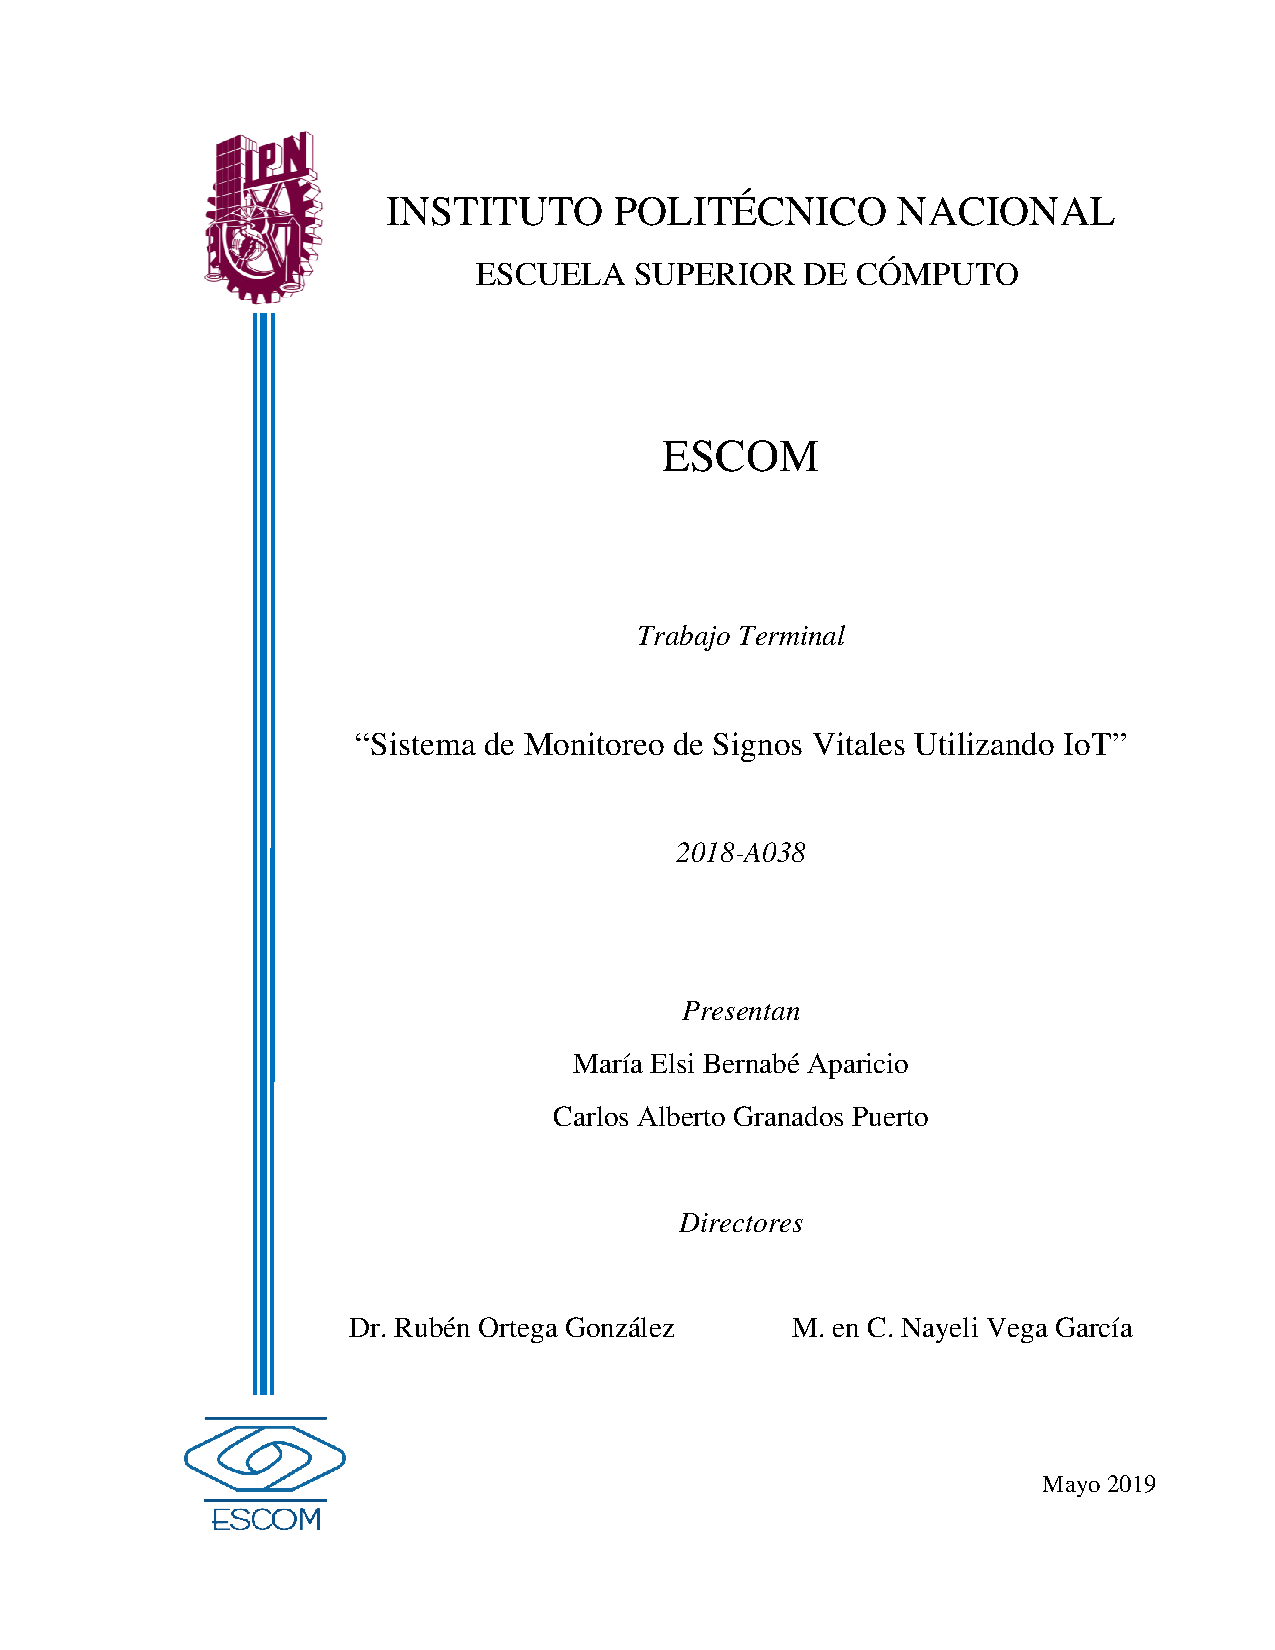
\includepdf[pages=1-1]{portadaTT.pdf}

%\maketitle
 
%=========================================================
% Hoja de revisión
%\makeDocInfo
%\vspace{0.5cm}
%\makeElemRefs
%\makeDocRefs
%\makeObservaciones[3cm]
%\vspace{0.5cm}
%\makeFirmas

%=========================================================
% Indices del documento
\frontmatter
% \LRCornerWallPaper{1}{cdt/theme/test4.png}
\tableofcontents
\listoffigures
\listoftables
\mainmatter

% Para esconder la información del documentador se descomenta el \hideControlVersion
% \hideControlVersion

% \cite{ab94}
 
%=========================================================
\chapter{Introducción}\label{chp:introduccion}
	\cfinput{Introduccion/introduccion}
   
%=========================================================
\chapter{Marco Teórico}\label{chp:marcoTeorico}
   \cfinput{MarcoTeorico/marcoteorico}
   
%=========================================================
\chapter{Análisis}\label{chp:analisis}
\cfinput{Analisis/analisis}
    
%=========================================================
\part{Diseño de la Estructura del Sistema}
\cfinput{DisenoEstructura/disenoEstructura}
\chapter{Modelo de Negocio}\label{chp:modeloNegocios}
\cfinput{ModeloNegocios/modelo}
\chapter{Modelo de Comportamiento}
\cfinput{ModeloComportamiento/comportamiento}
\chapter{Modelo de Interacción con el Usuario}
\cfinput{ModeloInteraccion/interaccion}


%=========================================================
\part{Implementación}
\chapter{Avances y pruebas}\label{chp:avancesPruebas}
\cfinput{AvancesPruebas/pruebas}




%=========================================================



%=========================================================
%\chapter{Modelo de negocio}\label{chp:modeloNegocios}
%    \cfinput{ModeloNegocios/modelo}
%%    \cfinput{ModeloNegocios/estructura}
%%    \cfinput{ModeloNegocios/registro}
%%    \cfinput{ModeloNegocios/informacion-base}
%%    \cfinput{ModeloNegocios/plan-accion}
%%    \cfinput{ModeloNegocios/seguimiento}
%%    \cfinput{ModeloNegocios/reglas}
%%    \cfinput{ModeloNegocios/indicadores-agua}
%%    \cfinput{ModeloNegocios/indicadores-residuos}
%%    \cfinput{ModeloNegocios/indicadores-energia}
%%    \cfinput{ModeloNegocios/indicadores-biodiversidad}
%%    \cfinput{ModeloNegocios/indicadores-ambienteEscolar}
%%    \cfinput{ModeloNegocios/indicadores-consumoResponsable}
%    
%===========================================================
%\chapter{Modelo de comportamiento}\label{chp:modeloComportamiento}
%  \cfinput{ModeloComportamiento/comportamiento}

%===========================================================
    	
%\chapter{Modelo de interacción con el usuario}\label{chp:modeloInteraccionUsuario}
%\cfinput{ModeloInteraccion/interaccion}

%---------------------------------------------------------------------
%\section{Interfaces del subsistema: Registro de escuelas}

%---------------------------------------------------------------------

%\section{Diseño de mensajes}
% \cfinput{ModeloInteraccion/mensajes}
%
%\setlength{\biblabelsep}{0.5em}
%\newcounter{MyBibCount}
%\makeatletter
%\renewcommand{\@biblabel}[1]{\stepcounter{MyBibCount}[\theMyBibCount]}
%\makeatother
%
\newpage
%%% Referencias
\renewcommand{\bibname}{Referencias}
%\bibliographystyle{apacite}
%\bibliography{referencias}

\cfinput{referencias}

\addcontentsline{toc}{chapter}{Referencias}

\end{document}
\grid
